\section{Problem Description} %%%%%%%%%%%%%%%%%%%%%%%%%%%%%%%%%%%%%%%%%%%%%%%%%%
\label{sec:probl}

The ideas and the library were motivated by our unsatisfactory experiences 
working with various C++ front-ends and program analysis 
frameworks~\cite{Pivot09,Phoenix,Clang,Liz}.
The problem was not in the frameworks per se, but in the fact that we had to use
the \emph{visitor design pattern}~\cite{DesignPatterns1993} to inspect, traverse, and 
elaborate abstract syntax trees to target languages. We found visitors 
unsuitable to express our application logic, surprisingly hard to teach 
students, and slow. Use of dynamic casts in many places, often nested,to 
answer simple structural questions, shows that the users 
preferd shorter, cleaner, and more-direct code to visitors, even at a high 
cost in performance.

A lot has been written about the visitor design pattern~\cite{DesignPatterns1993,Zenger:2001,Oliveira08}. 
Its advantages include \emph{extensibility of functions}, \emph{speed}, and, \emph{being a library solution}. Nevertheless, the solution 
is still \emph{intrusive}, \emph{specific to hierarchy}, and requires a lot of 
\emph{boilerplate code} to be written. It also introduces \emph{control 
inversion}, and, most importantly, -- \emph{hinders extensibility} of classes.
Interestingly, as bad as visitors are, they are only trying to solve a larger 
problem in the context of object-oriented languages.

%Expression problem is a problem of supporting in a programming language modular 
%extensibility of both data and functions at the same time. Functional languages
%allow for easy addition of new functions at the expense of disallowing new data
%variants. Object-oriented languages allow for easy addition of new variants at 
%the expense of disallowing new functions. Many attempts have been made to 
%resolve this dilema in both camps, nevertheless no universally accepted solution 
%that is modular, open and efficient has been found.

%Visitor Design Pattern has became de-facto standard in dealing with expression 
%problem in many industry-strength object-oriented languages because of two 
%factors: its speed and being a library solution. It comes at the cost of 
%restricting extensibility of data, increased verbosity and being hard to teach 
%and understand, but nevertheless, remains the weapon of choice for interacting 
%with numerous object-oriented libraries and frameworks. 

Conventional algebraic datatypes, as found in most functional languages,
allow for easy addition of new functions on existing data types.
But they fall short in extending data types themselves 
(e.g. with new constructors), 
which requires modifying the source code. Object-oriented languages, on the 
other hand, make data type extension trivial through inheritance;
but the addition of new functions operating on these classes typically
requires changes to the class definition \cite{Cook90,exprproblem}. 
Classes differ from algebraic data  types in two important ways: they
are \emph{extensible}, for new variants can be added by inheriting from
the base class.  They are \emph{hierarchical} and thus typically
\emph{non-disjoint} since variants can be inherited from other variants
and form a subtyping relation between themselves~\cite{Glew99}. 
On the contrary, algebraic data types form \emph{closed} and \emph{disjoint}
sets of variants. Some functional languages e.g. ML2000~\cite{ML2000}
and its predecessor, Moby, were experimenting with 
\emph{hierarchical extensible sum types}, which are closer to 
object-oriented classes then algebraic data types are, but, 
interestingly, they did not provide pattern matching facilities on them!

Zenger and Odersky later refined the expression problem in the context of 
independently extensible solutions~\cite{fool12} as a challenge to find an 
implementation technique that satisfies the following requirements:

\begin{itemize}
\setlength{\itemsep}{0pt}
\setlength{\parskip}{0pt}
\item \emph{Extensibility in both dimensions}: It should be possible to add new 
      data variants, while adapting the existing operations accordingly. It 
      should also be possible to introduce new functions. 
\item \emph{Strong static type safety}: It should be impossible to apply a 
      function to a data variant, which it cannot handle. 
\item \emph{No modification or duplication}: Existing code should neither be 
      modified nor duplicated.
\item \emph{Separate compilation}: Neither datatype extensions nor addition of 
      new functions should require re-typechecking the original datatype or 
      existing functions. No safety checks should be deferred until link or 
      runtime.
\item \emph{Independent extensibility}: It should be possible to combine 
      independently developed extensions so that they can be used jointly.
\end{itemize}

\noindent
Object-oriented languages further complicate the matter with the fact that 
data variants are not necessarily disjoint and may form subtyping relationships  
between themselves. We thus introduced an additional requirement based on 
Liskov substitution principle~\cite{Lis87}:

\begin{itemize}
\setlength{\itemsep}{0pt}
\setlength{\parskip}{0pt}
\item \emph{Substitutability}: Operations expressed on more general data variants
      should be applicable to more specific ones that are in a subtyping relation 
      with them.
\end{itemize}

%Depending on the semantics of the language's subtyping relation, 
%substitutability requirement may turn pattern matching into an expensive 
%operation. OCaml, for example, that uses structural subtyping on its object 
%types, does not offer pattern 

\noindent
We will refer to a solution that satisfies all of the above requirements as \emph{open}. 
Numerous solutions have been proposed to dealing with the expression problem in both 
functional and object-oriented camps, but very few are truly open, while 
none has made its way into one of the mainstream languages. We refer the reader 
to Zenger and Odersky's original manuscript for a discussion of the 
approaches~\cite{fool12}. Interestingly, most of the discussed object-oriented 
solutions were focusing on the visitor design pattern~\cite{DesignPatterns1993}, 
which even today seems to be the most commonly used approach to dealing with the 
expression problem in practice.

\subsection{Type Switch}

This section generalizes pattern matching of closed algebraic datatype values
to case analysis of hierarchical and extensible datatype values.
We call \emph{type switch} a control structure taking either an object
descriptor (pointer of reference), called \emph{subject}, and uncovers a 
descriptor to a full object of a type present in the list of case 
clauses. Similar control structures exist in many programming languages and 
date back to at least Simula's Inspect statement~\cite{Simula67}.

Consider a class \code{B} and a set of classes \code{Di} directly 
or indirectly inherited from it. Having an instance of class \code{D} referenced 
by a variable \code{base} of static type \code{B&}, a hypothetical type switch 
statement, not currently supported by C++, can look as following:

\begin{lstlisting}[keepspaces]
switch (base) { case D1: s1; ... case Dn: sn; }
\end{lstlisting}

\noindent and can be given numerous plausible semantics:

\begin{itemize}
\setlength{\itemsep}{0pt}
\setlength{\parskip}{0pt}
\item \emph{First-fit} semantics will evaluate the first statement $s_i$ such 
      that $D_i$ is a base class of $D$
\item \emph{Best-fit} semantics will evaluate the statement corresponding to the 
      most derived base class $D_i$ of $D$ if it is unique (subject to 
      ambiguity)
\item \emph{The-only-fit} semantics will evaluate statement $s_i$ if $D_i=D$.
\item \emph{All-fit} semantics will evaluate all statements $s_i$ whose guard 
      type $D_i$ is a subtype of $D$ (order of execution has to be defined)
\item \emph{Any-fit} semantics might choose non-deterministically one of the 
      statements enabled by all-fit
\end{itemize}

\noindent
The list is not exhaustive and depending on a language; any of these semantics can be a plausible choice. Functional languages, for 
example, often prefer first-fit, while object-oriented languages would typically 
be inclined to best-fit semantics. The-only-fit semantics is traditionally seen 
in procedural languages like C and Pascal to deal with discriminated union types. 
All-fit and any-fit semantics might be seen in languages based on predicate 
dispatching~\cite{ErnstKC98} or guarded commands~\cite{EWD:EWD472}, where a 
predicate can be seen as a characteristic function of a type, while logical 
implication can be seen as subtyping.

\subsection{Open and Efficient Type Switching}
\label{sec:poets}

The closed nature of algebraic data types allows for 
their efficient implementation. 
The traditional compilation scheme assigns unique 
tags to every variant of the algebraic data type and pattern matching is then 
simply implemented with a jump table over all tags. A number of issues in 
class hierarchies makes this extremely efficient approach infeasible:

\begin{itemize}
\setlength{\itemsep}{0pt}
\setlength{\parskip}{0pt}
\item \emph{Extensibility} implies that the compiler may not know the exact set 
      of all derived classes till link-time (due to \emph{separate compilation}) 
      or even run-time (due to \emph{dynamic linking}).
\item \emph{Substitutability} requirement implies that we should be able to 
      match tags of derived classes against case labels representing tags of 
      base classes.
\item Presence of \emph{multiple inheritance} might require pointer adjustments 
      that are not known at compile time (e.g. due to virtual base class or 
      cross-casting).
\end{itemize}

\noindent
In some cases the substitutability requirement can be satisfied by obtaining 
the base class' tag from a derived one first and then performing the jump. 
This will work as long as we have only base classes in the case clauses.
Derived classes that have to be treated separately from the rest of their 
siblings, will essentially be indistinguishable from them.

When tags are not chosen arbitrarily but to reflect the subtyping relation of the 
underlying hierarchy (e.g. certain bit set for certain base class), the assumed 
structure of tags is likely to make the set of tags sparse. On one side this 
decreases the number of representable hierarchies and thus hinders openness, 
while on the other forces the compiler to use a decision tree instead of a jump 
table to implement the switch. The former was consistently slower than the 
latter one in our experience, even though the opposite was noted on some 
architectures for small number of cases~\cite[\textsection 4]{garrigue-98}.

Instead of starting with an efficient solution and trying to make it open, we 
start with an open solution and try to make it efficient. The following 
cascading-if statement implements the first-fit semantics for our type switch in 
a truly open fashion:

\begin{lstlisting}
if (D1* derived = dynamic_cast<D1*>(base)) { s1; } else
if (D2* derived = dynamic_cast<D2*>(base)) { s2; } else
...
if (Dn* derived = dynamic_cast<Dn*>(base)) { sn; }
\end{lstlisting}

\noindent
Its main drawback is performance: a typical 
implementation of \code{dynamic_cast} takes time proportional to the 
distance between base and derived classes in the inheritance tree~\cite{XXXXX}.
What is worse, is that the time to uncover the type in the $i^{th}$ case clause 
is proportional to $i$, while failure to match will always take the longest. 
This linear increase can be seen in the Figure~\ref{fig:DCastVis1}, where 
the above cascading-if was applied to a flat hierarchy encoding an algebraic 
data type with 100 variants. The same type-switching functionality implemented 
with the visitor design pattern took only 28 cycles regardless of the case.
\footnote{Each case $i$ was timed multiple times, thus turning the experiment 
into a repetitive benchmark described in \textsection\ref{sec:eval}. In a more
realistic setting, represented by random and sequential benchmarks, the cost of 
double dispatch was varying between 52 and 55 cycles.}
This is more than 3 times faster than the 93 cycles it took to uncover even the 
first case with \code{dynamic_cast}, while it took 22760 cycles to uncover the 
last.

\begin{figure}[htbp]
  \centering
    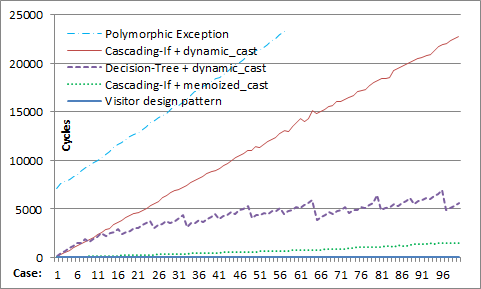
\includegraphics[width=0.47\textwidth]{DCast-vs-Visitors1.png}
  \caption{Type switching based on na\"ive techniques}
  \label{fig:DCastVis1}
\end{figure}

Seeing several solutions whose time increases with the position of the case 
clause in the type switch, one may wonder how many such clauses a typical 
program might have. A program dealing with abstract syntax trees in 
Pivot~\cite{Pivot09} that we implemented using our pattern-matching library had 
8 match statements with 5, 7, 8, 10, 15, 17, 30 and 63 case clauses, 
respectively. With Pivot having the smallest number of node kinds among the 
compiler frameworks we had a chance to work with, we expect a similar or larger 
number of case clauses in other compiler applications.

When the class hierarchy is not flat, the above cascading-if can be replaced 
with a decision tree that tests base classes first and thus eliminates many of 
the derived classes from consideration -- an approach used by Emir to deal with 
type patterns in Scala~\cite[\textsection 4.2]{EmirThesis}. The intent is to 
replace a sequence of independent dynamic casts between classes that are far 
from each other in the hierarchy with nested dynamic casts between classes that 
are close to each other. Another advantage is the possibility to fail early. 
As can be seen from Figure~\ref{fig:DCastVis1} under ``Decision-Tree + 
dynamic\_cast'', when applicable, the optimization can be very useful. The class
hierarchy for this timing experiment formed a perfect binary tree with 
classes number 2*N and 2*N+1 derived from a class with number N. The hierarchy 
also explains the repetitive pattern of timings.

The above solution either in a form of cascading-if or as a decision tree can be 
significantly improved by lowering the cost of a single \code{dynamic_cast}. 
We devised an asymptotically constant version of this operator, called
\code{memoized_cast}~\cite{TR}, which memoizes the outcome of a call to 
\code{dynamic_cast} using techniques from \textsection\ref{sec:copc}. As can be 
seen from the graph titled ``Cascading-If + memoized\_cast'', it speeds up the 
above cascading-if solution by a factor of 18 on average, as well as outperforms 
the decision-tree based solution with dynamic\_cast for a number of case clauses 
way beyond those that can happen in a reasonable program. The slowest 
implementation in the chart is based on exception handling facilities of C++ and 
is described in technical report~\cite{TR}.

The approach of Gibbs and Stroustrup~\cite{FastDynCast} employs divisibility of 
numbers to obtain a tag allocation scheme capable of performing type testing in 
constant time. Extended with a mechanism for storing offsets required for 
this-pointer adjustments, the technique can be used for extremely fast dynamic 
casting. We handcrafted this technique on the above flat 
and binary-tree hierarchies and redid the timing experiments from 
Figure~\ref{fig:DCastVis1} for comparison. The results are 
presented in Figure~\ref{fig:DCastVis2}. We retained 
``Visitor Design Pattern'' and ``Cascading-If + memoized\_cast'' timings from 
Figure~\ref{fig:DCastVis1} unchanged for reference. Note that the Y-axis has been scaled-up 
140 times, making the slope of ``Cascading-If + memoized\_cast'' timings much steeper.

\begin{figure}[htbp]
  \centering
    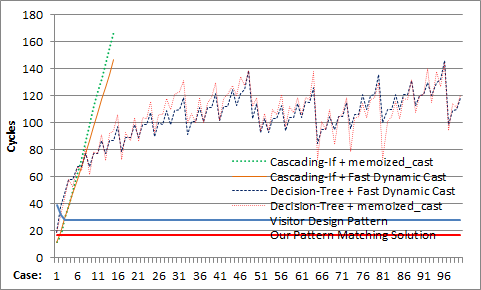
\includegraphics[width=0.47\textwidth]{DCast-vs-Visitors2.png}
  \caption{Type switching based on the fast dynamic cast of Gibbs and Stroustrup~\cite{FastDynCast}}
  \label{fig:DCastVis2}
\end{figure}

%As can be seen from the figure the use of our memoized\_cast implementation can 
%get close in terms of performance to the fast dynamic cast, especially 
%when combined with decision trees. An important difference that cannot be seen 
%from the chart, however, is that the performance of memoized\_cast is 
%asymptotic, while the performance of fast dynamic cast is guaranteed. This 
%happens because the implementation of memoized\_cast will incur an overhead of 
%a regular dynamic\_cast call on every first call with a given most derived type. 
%Once that class is memoized, the performance will remain as shown. Averaged over 
%all calls with a given type we can only claim we are asymptotically as good as 
%fast dynamic cast.

Unfortunately fast dynamic casting is not truly open as the structure of tags 
required by the scheme limits the number of classes it can handle. 
%A 32-bit integer is estimated to be able to represent 7  
%levels of a class hierarchy that forms a binary tree (255 classes), 6 levels of 
%a similar ternary tree hierarchy (1093 classes) or just one level of a hierarchy 
%with 9 base classes -- multiple inheritance is the worst case scenario of the 
%scheme that quickly drains its allocation possibilities. 
The presence of class extensions in \emph{Dynamically Linked Libraries} (DLLs) 
will also require an integration effort to make sure different DLLs are not 
reusing prime numbers in a way that might result in an incorrect dynamic cast.
Interestingly, while suitable for type testing and type switching with decision 
trees, the fast dynamic cast approch is not suitable for type switching with 
jump tables: computing the tag of a base class will have to decompose the 
derived tag into primes.

A number of other constant-time techniques for class-membership testing is 
surveyed by Gil and Zibin~\cite[\textsection 4]{PQEncoding}. They are intended 
for type testing, and thus will have to be combined with decision trees 
for type switching, resulting in similar to fast dynamic cast performance. 
They too assume access to the entire class hierarchy at compile time and thus 
are not open.

To summarize, truly open and efficient type switching is a non-trivial problem. 
The approaches we found in the literature were either open or efficient, 
but not both. Efficient implementation was typically achieved by sealing the 
class hierarchy and using a jump table on sequential tags. Open implementations 
were resorting to type testing and decision trees. 
We are unaware of any efficient tag allocation scheme that can be used in a 
truly open scenario.
